\documentclass[11pt]{article}

\usepackage{fullpage}
\usepackage{graphicx}
\usepackage{hyperref}

\title{Evolving robots to play capture the flag}
\author{Uriel Mandujano and Daniel Redelmeier}
\date{} %don't display the current date

\begin{document}

\maketitle

\begin{abstract}

  In nearly all videogames, designing smart and complex artificial agents is necessary to ensure a fun player experience. In this experiment, we attempt to meet this challenge by training robots to develop effective strategies in a simple two-player game similar to Capture the Flag. The robots start on opposite ends of a field, and must attempt to reach a flag in the center and return it to their base without being touched. The catch is that any robot carrying the flag can only move at 70\% speed, enabling the flag to be stolen. Stealing the flag from the opponent grants a significant advantage: the flag is transferred and the previous flag-carrier is teleported back to their base. We implemented the game in the Pyrobot simulator, and used separate feedforward neural networks to control two robots playing against each other. Using this model, we evolved the robots to continuously improve on their performance through competitive coevolution in NEAT. We hypothesized several strategies that might develop. A straight offensive strategy would involve grabbing the flag as quickly as possible, and trying to bring it back to the base before being caught. A more defensive strategy might make use of the captuing mechanism to steal the flag after the opponent had grabbed it. Our results showed that both strategies evolved at different times (first offensive, and later defensive), as well as others. Although the final best strategies were straightforward and predictable from a gameplay perspective, we believe our setup has strong potential; further experimentation and refinement could produce robots that are worthy of human opponents. Moreover, this experiment shows that competitive coevolution can be used to improve videogame AI as a whole with relatively minimal human input.
  
\end{abstract}

\section{Introduction}

  Capture the Flag is a children's game usually played outside. A large playing area is divided in two, with each region being a safe area for one team but not the other. Both teams hide an object -- the ``flag" -- somewhere in their region before the game begins. The object of the game is to find the opponent's flag and bring it back to the safe zone before the other team. If an individual is tagged outside of their zone while looking for or carrying the flag, they must return to their side of the field and drop the flag if they have it. Some online versions of Capture the Flag exist, such as TagPro (see \url{tagpro.koalabeast.com}).
  
  In our simplified version of the game, we ran the same competitive coevolution algorithm on two populations of robot brains to improve overall performance. Due to the competitive nature of the game, a robot tended to have a higher fitness if it was closer to winning the game. The population was capped, so phenotypes of fitter individuals would be more present in the next generation. When evaluating one robot, the brain of its competitor was set as the best-performing opponent phenotype from the previous generation, which ensured that both robots had to develop new strategies to succeed. We performed competitive coevolution using Neuroevolution of Augmenting Topologies (NEAT), ``a method for evolving artificial neural networks with a genetic algorithm," developed by Kenneth O. Stanley in 2002 \cite{NEAT_website}.
  
We are not the first to run such experiments.  Stanley and Miikulainen ran competitive coevolution tests to create a ``Robot Duel", a simulated conflict between two distinctly evolving populations \cite{NEAT}. Pitting two individuals against each other addresses the issue of getting stuck in local optima that can occur in standard back-propagation for neural networks.  As soon as one robot has evolved a sufficiently dominant strategy, the other robot works to evolve a more dominant strategy, creating a cycle that could continue indefinitely. Another distinct advantage to using a co-evolution strategy is it provides a basis for studying complexification. The network begins with a minimal number of nodes and adds more nodes and connections as strategies are created. In their Robot Duel, they expected to never encounter an entirely dominant strategy simply because evolution is continuous.  Their results comfirmed that continuous evolution results in increasingly sophisticated strategies.

Another study investigating coevolution was done by Floreano and Nolfi \cite{red_queen}. They use pursuit-evasion goals to explore the dynamics of learning. Pursuit-evasion is a competition that models natural occurences, e.g. a cat and mouse.  In our own tests, we experimented with two different fitness functions: one that only offered a positive reward upon the accomplishment of tasks; the other subtracted fitness from an individual if it lost an encounter with the opponent.  The latter fitness function is more akin to Floreano and Nolfi's study and we were curious to see how impactful the change would be. They never observed the absolute dominance of one strategy. In fact, some individuals of `more evolved' generations would lose to those of earlier, `less evolved' generations.  Granted, they compared the most recent generation's individuals to those in simulations ten generations earlier.  But even with this caveat, no strategies  that developed in the most recent simulations exhibited more complex solutions. 

Miller and Cliff also experimented with coevolution and pursuit-evasion \cite{pursuit}. They note that if in a simulation, the individuals benefit from being together, they would evolve in a manner more likely to pursue and keep track of each other.  It they benefitted from being seperate, they would evolve to keep their distance at all times.  If, however, one individual benefitted from an encounter with the other, some sort of cat and mouse game would develop. Indeed, this is similar to Floreano and Nolfi's study, and is what we were attempting to replicate in our experiments with the detrimental fitness function.

\section{Experiments}

\begin{figure}[h]
\begin{center}
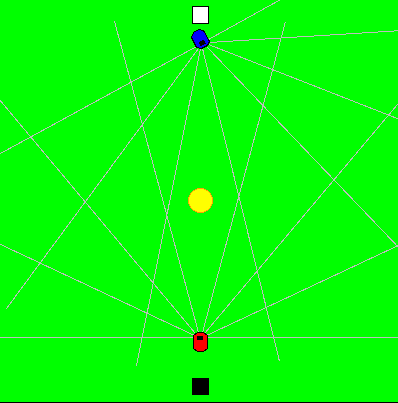
\includegraphics[scale=0.5]{Screenshot_-_030714_-_00_15_04.png}
\end{center}
\caption{This picture shows the Pyrobot playing field after a sample trial has just begun. Both robots have already begun to leave their respective bases and move toward the flag, coded as a light source in Pyrobot. The robots have access to their front sonar and light-detection sensor values, as well as 8 other inputs.}
\label{setup}
\end{figure}

Our experiment setup consisted of a 10-by-10 playing field modelled in the Pyrobot simulator. A red and and a blue robot start on opposite sides of the field equidistant from the flag in the center, just in front of their bases (the blue robot had the white base, and the red robot had the black base). The rules of the game were simple:
\begin{itemize}
  \item Both robots could move anywhere on the field, although both bases were impassable
  \item If the robot touched the flag, it immediately gained possession while its maximum speed was reduced by 30\%
  \item If one robot came within 0.75 units of the flag-carrying robot, the flag immediately changed possession, and the initial-flag carrier was teleported back to their starting position
  \item Most trials ran for 125 steps. However, if either robot returned the flag to their base, the trial ended immediately
\end{itemize}

The robots had 11 total input values and three hidden nodes to determine motor output: the front right and left light sensor input, the front center sonar sensor input, two booleans that indicated whether the blue or red robot had the flag, the robot's x and y distance from its base and its heading, and  its x and y distance from the opponent as well as the opponent's heading.

Our fitness function to evaluate a robot's performance was more complex, and gave greater rewards scaling with how close a robot was to achieving the main objective. Initially, the fitness was determined by how close a robot's final position was to the flag, if neither competitor retrieved it. When the flag began to be picked up, different fitnesses were calculated to encourage robots to return the flag if they had it, and pursue their opponent if not. Due to the layered quality of our function, we coded it using several conditional statments:

\begin{verbatim}
  if the robot being evaluated does not win the game in 125 time steps:
 
     if neither robot ever grabs the flag:
        fitness = 8 - distance from flag
     if the robot never had the flag, but its opponent did:
        fitness = 16 - distance from opponent   
     if the robot had the flag, but its opponent has it at the end of the trial:
        fitness = 20 - distance from opponent  
     if the robot has the flag at the end of the trial:
        fitness = 24 - distance from home base
  
  else:
     fitness = 24
\end{verbatim}

Each robot was evaluated twice, so the maximum possible fitness (the sum of the fitness for each evaluation) was 48. Using this setup, we ran three similar experiments over three runs each. All runs were done with a population of 40 for each robot over 15 generations, which we found to be sufficient for obtaining useful results. Our first test used the base code and the default evolution parameters. The second test altered the fitness function to punish a robot with -6 fitness if it ever lost the flag. Our final test used the initial fitness function, but increased the probability of adding connections and nodes from 5\% to 10\% and 3\% to 6\% respectively.

\section{Results}

\begin{figure}[h]
\begin{center}
\fbox{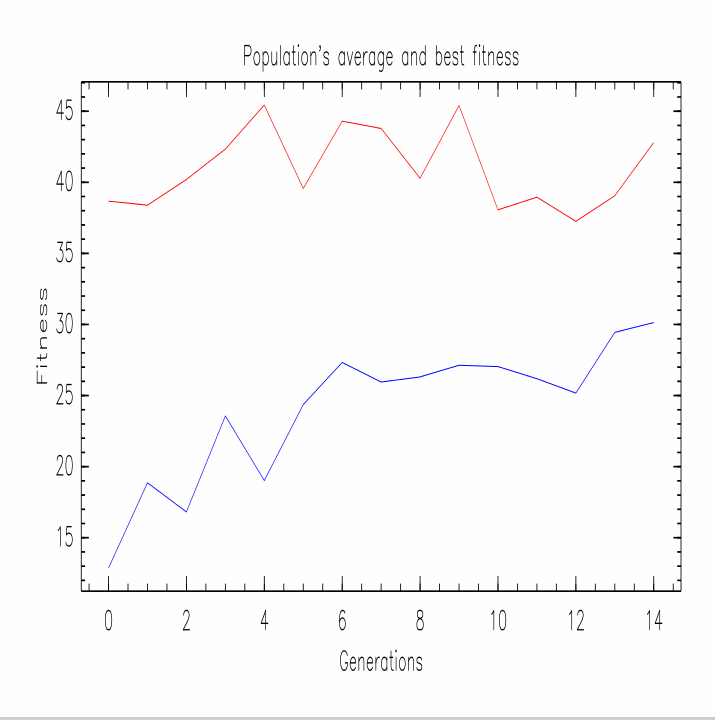
\includegraphics[scale=0.3]{Screenshot_-_030614_-_11_10_17.png}}
\fbox{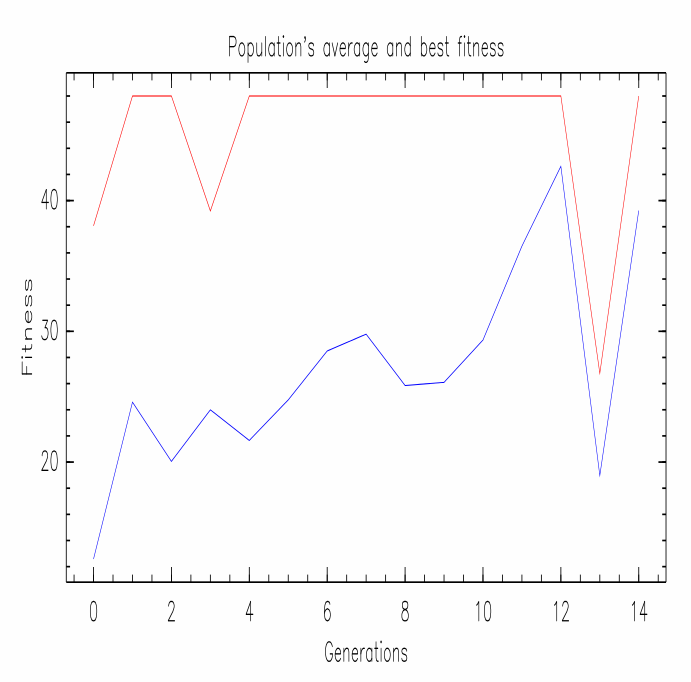
\includegraphics[scale=0.315]{Screenshot_-_030614_-_11_10_46.png}}
\end{center}
\caption{Both graphs show the average and best fitness progression for trial 2 of the first experiment. The average fitness (in blue) is shown for the red robot on the left and the blue robot on the right, and there is a clear upward trend in performance for both. We discovered that the sharp fall in the blue robot's fitness at generation 13 was likely caused by a mostly defensive blue population facing off against a red phenotype that likewise played defensively. When we evaluated that generation specifically, we found that both robots were reluctant to grab the flag, which explains the decline in fitness. This was remedied in the subsequent generation, as a more offensive blue population had evolved.}
\label{experiment1fitness}
\end{figure}

\begin{figure}[h]
\begin{center}
\fbox{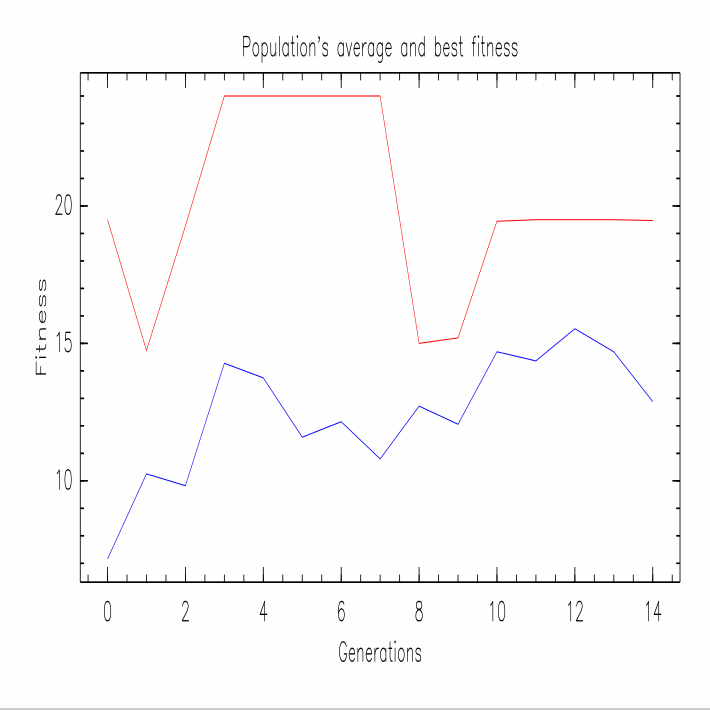
\includegraphics[scale=0.295]{40.png}}
\fbox{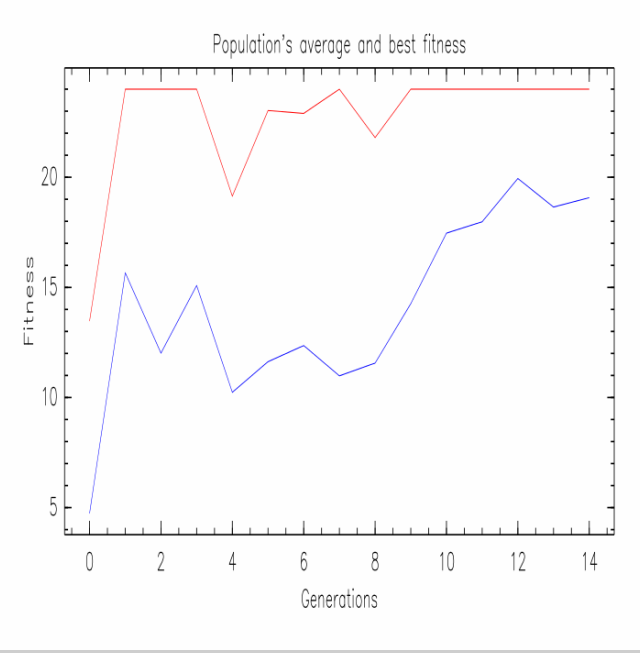
\includegraphics[scale=0.32]{34.png}}
\fbox{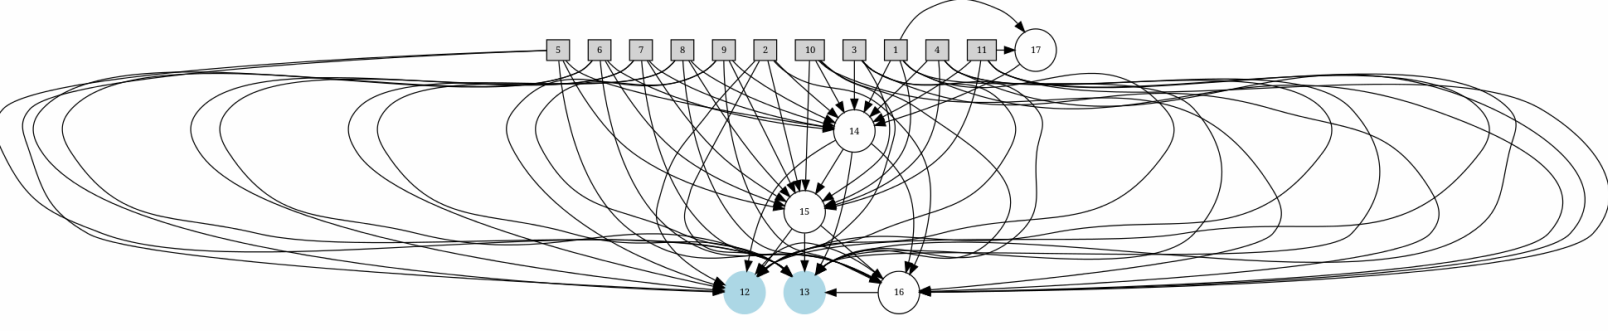
\includegraphics[scale=0.26]{cooler_network.png}}
\end{center}
\caption{Like Figure 2, the graphs show the average and best fitness progression for the red (top-left) and blue (top-right) robts. These graphs came from trial 3 of the second experiment. As expected, there is still a net increase in fitness for each robot. Interestingly, the blue robot developed a unique strategy that we did not expect or find in other trials. Beginning in Generation 9, the blue robot would circle to the left of the red robot instead of heading straight for the flag. When the red robot grabbed the flag and began to rotate back to its base, the blue robot was already in a position to intercept. This is where the robot's strategy began to disintegrate, although this may have been remedied with more generations. The most-fit blue topology from Generation 12 is shown below the graphs. Note the addition of a hidden node (17) that was not present at the beginning.}
\label{experiment1fitness}
\end{figure}

Our results for all three experiments showed general increases in fitness for both the red and blue robots as evolution progressed. Specific evolutionary developments are shown in Figures 2 and 3 for Experiments 1 and 2. Unfortunately, none of the trials in Experiment 3 had particularly interesting results, and the average fitness increase was was lowest of all the experiments. This might have been different if we ran our trials for more generations, as the additional nodes and connections might have had a more positive impact. This is quite plausible, since complexifying coevolution in NEAT has already been shown to be effective.

\section{Discussion}

Our results add further evidence supporting the effectiveness of using competitive coevolution to create solutions to problems in AI. We consistently saw the fitness improve thoughout each trial.  For example, early successful phenotypes tended to compete in a mad dash to the flag in the center.  Later on, we saw both robots become more patient and hesitate before going for the flag.  Another strategy was to wait for the opponent to obtain the flag before "capturing the flag" and resetting their position. Further testing with longer trial runs may yield more interesting and unforseen strategies and the development of complex strategies falls in line with the current research \cite{NEAT}.  Initially the robots develop simple strategies corresponding to few nodes and connections. Building off of these networks creates foundations for more creatively complex strategies. 

Overall, we believe that our experiments were successful in developing adaptive strategies without the need to hard-code functions to determine motor output. If we are able to run more generations and develop better topologies, we may see the rise of robots that can reasonably compete against a human-controlled opponent. We could then evaluate and evolve the robots based on interactions with humans, and reveal insights into human tendencies for strategies in the game. We believe that competitive coevolution should be applied to other challenged in AI development outside of the Pyrobot simulation.

\section{Acknowledgements}

Our experiment was more complicated than initially intended, and we could not have done it by ourselves. We would like to thank Lisa Meeden for providing the base code to perform competitive coevolution in NEAT on a Pyrobot simulation, as well as guidance on the project. Additionally, we would  like to thank Joe Boninger for showing us a trigonometric algorithm to help the robots make better turning decisions. Finally, thanks to Ben Xie and Tyler Zon for helping us create separate files that ran our tests outside of the simulation window, which allowed us to perform more trials in a shorter amount of time.

\begin{thebibliography}{1}

  \bibitem{red_queen} Dario Floreano and Stefano Nolfi, God save the red queen! competition in co-evolutionary robotics. {\em Evolutionary Computation}, 5, 1997.

  \bibitem{pursuit}  Geoffrey F. Miller and Dave Cliff, Co-evolution and pursuit and evasion i: Biological and game-theoretic foundations. 1994.

  \bibitem{NEAT} Kenneth O. Stanley and Risto Miikkulainen, Competitve coevolution through evolutionary complexification {\em HJournal of Artifical Intlelignce Research}, 21, 2004.
  
  \bibitem{NEAT_website} Kenneth O. Stanley. The NeuroEvolution of Augmenting Topologies (NEAT) Users Page. {\em NEAT Software FAQ}, 2013. \url{http://www.cs.ucf.edu/~kstanley/neat.html}


  \end{thebibliography}

\end{document}
